\documentclass[arhiv]{../izpit}
\usepackage{fouriernc}
\usepackage{tikz}
\usepackage{censor}
\usepackage{paralist}
\usepackage{eurosym}
\usepackage{url}

\begin{document}

\izpit{Programiranje I: 2.\ izpit}{13.\ sušec v letu Gospodovem 2014}{
  Čas reševanja je 150 minut.
  Doseženih 100 točk šteje za maksimalno oceno.
  Veliko uspeha!
}

%%%%%%%%%%%%%%%%%%%%%%%%%%%%%%%%%%%%%%%%%%%%%%%%%%%%%%%%%%%%%%%%%%%%%%
\naloga[Plače, 10 + 10 + 10 točk]
V nekem uspešnem slovenskem podjetju so zaposleni urejeni hierarhično. Vsakdo razen direktorja ima natanko enega nadrejenega. Vsak uslužbenec ima lahko pod seboj največ dva podrejena (levega in desnega). Primer takšne hierarhije (številke so njihove plače):
$$
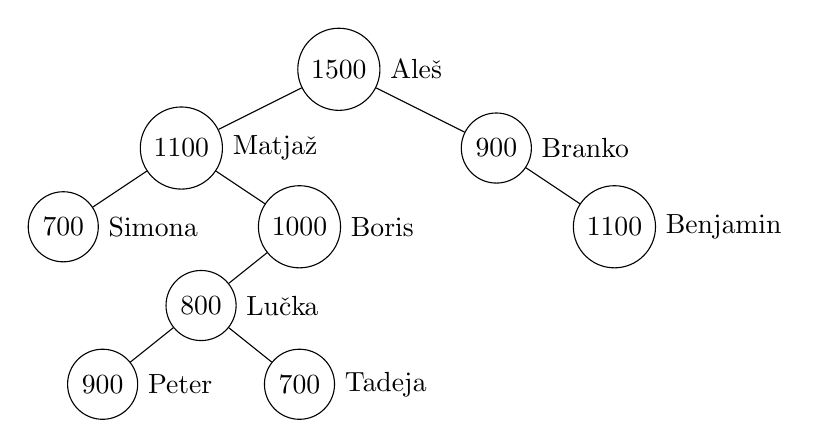
\begin{tikzpicture}[level distance=1cm,
    level 1/.style={sibling distance=4.0cm},
    level 2/.style={sibling distance=3cm},
    level 3/.style={sibling distance=2.5cm}
    ]
    \node[circle, draw, label=0:Aleš] (d) {1500}
      child {node[circle, draw, label=0:Matjaž] {1100}
        child {node[circle, draw, label=0:Simona] {700}}
        child {node[circle, draw, label=0:Boris] {1000}
          child {node[circle, draw, label=0:Lučka] {800}
             child {node[circle, draw, label=0:Peter] {900}}
             child {node[circle, draw, label=0:Tadeja] {700}}
          }
          child[missing]{}
        }
      }
      child {node[circle, draw, label=0:Branko] {900}
        child[missing] {} 
        child {node[circle, draw, label=0:Benjamin] {1100}}
      }; 
  \end{tikzpicture}
$$

V tem podjetju imajo zelo močen sindikat. Sindikalisti so ugotovili, da višine plač niso pravične. Nedopustno je, da imajo nekateri podrejeni višje plače od svojih nadrejenih! Zato sindikat zahteva, da mora imeti vsak zaposleni vsaj za 100 \euro{} višjo plačo od kateregakoli svojega podrejenega.

Direktor bi rad analiziral podatke, preden se spusti v pogajanja s sindikalisti. Podatke o plačah zaposlenih je shranil v podatkovno strukturo \texttt{Drevo}, ki je že implementirana. V vozliščih so shranjeni podatki o plačah zaposlenih (atribut \verb+placa+) in njihova imena (atribut \verb+ime+).

\podnaloga[10 točk]
Direktorja zanima, koliko dodatnega denarja bi potreboval vsak mesec, če bi ugodil zahtevam sindikata. Želi, da sestavite funkcijo \texttt{naloga1a(self)}, ki vrne skupno vsoto denarja, ki bi ga potreboval za odpravo krivic. Primer (če \texttt{d} ustreza zgornji sliki):
%
\begin{verbatim}
>>> d.naloga1a()
700
\end{verbatim}
Komentar: Lučka bi po novem prejemala 1000 \euro, ker dobiva Peter 900 \euro. Zaradi Lučke bi moral  Boris prejemati 1100 \euro. Zaradi Borisa pa bi moral Matjaž prejemati 1200 \euro. Branko bi zaradi Benjamina moral prejemati 1200 \euro. Vsota vseh povišic znaša 700 \euro.

\podnaloga[10 točk]
Direktor bi sindikaliste rad prepričal, da se razburjajo po nepotrebnem. Rad bi imel seznam imen vseh tistih uslužbencev, ki bi prejeli povišice. (Od vseh takih bo namreč pridobil pisne izjave, da so zadovoljni s svojo plačo.) Napišite funkcijo \texttt{naloga1b(self)}, ki vrne množico imen vseh zaposlenih, ki bi prejeli povišico. Primer:
%
\begin{verbatim}
>>> d.naloga1b()
{'Lučka', 'Boris', 'Branko', 'Matjaž'}
\end{verbatim}

\podnaloga[10 točk]
Po večtedenskih pogajanjih s sindikatom je imel direktor poln k\censor{urac} vsega, zato je udaril po mizi! Odločil se je, da bo najprej vsem plače zmanjšal na ``minimalce'', potem pa bo povišal plače na način, ki ga predlaga sindikat. Tako bo volk sit in koza cela. Napišite funkcijo \texttt{naloga1c(self)}, ki vrne skupno vsoto denarja, ki bi ga na ta način prihranil vsak mesec (glede na trenutne plače). ``Minimalec'' znaša 500 \euro.

Primer:
%
\begin{verbatim}
>>> d.naloga1c()
3100
\end{verbatim}

%%%%%%%%%%%%%%%%%%%%%%%%%%%%%%%%%%%%%%%%%%%%%%%%%%%%%%%%%%%%%%%%%%%%%%
\naloga[Podnapisi, 15 + 20 točk]

Franci zelo rad gleda filme. Ker ne razume tujih jezikov, si s strani \url{www.podnapisi.net} sname
podnapise. Datoteke s podnapisi (ki imajo končnico \verb+.srt+) so takšne oblike\footnote{Zgled je iz filma \emph{Kajmak in marmelada}.}:
\begin{verbatim*}
1
00:08:51,520 --> 00:08:53,317
Pa je šla nevesta!

2
00:14:03,920 --> 00:14:08,357
Jebi ga, jaz bi ti pomagal,
samo šofer, Slovenec...

3
01:18:07,640 --> 01:18:12,589
Ima ta tvoja Špela na desni
joški materino znamenje? Ima?!

4
01:18:17,040 --> 01:18:22,194
Jebi ga, Božo.
Umiri malo žogo.
\end{verbatim*}
Za nas bo beseda \emph{podnapisi} pomenila zaporedje manjših enot, ki jim bomo rekli \emph{napisi}. Napisi so med seboj ločeni s po eno prazno vrstico. Vsak napis je sestavljen iz treh ali več vrstic. V prvi vrstici je zaporedna številka napisa, v drugi čas trajanja, od tretje dalje pa je besedilo.

Ker podnapise delajo amaterji, se včasih zgodi, da na neki točki začnejo podnapisi zaostajati ali pa prehitevati.
To gre Franciju zelo na k\censor{urac}. Če boste sestavili program, ki bo sposoben podnapise
popraviti, se vam obeta gajba\ldots

\podnaloga[15 točk]
Sestavite funkcijo \texttt{naloga2a(h, m, s, milis)}, ki dobi čas v urah, minutah, sekundah in milisekundah ter ga preračuna v milisekunde. Sestavite še funkcijo \texttt{naloga2b(milis)},
ki naredi ravno obratno, tj. dobi čas v milisekundah in ga preračuna v ure, minute, sekunde in milisekunde. Primer:
\begin{verbatim}
>>> naloga2a(1, 18, 7, 640)
4687640
>>> naloga2b(4687640)
(1, 18, 7, 640)
\end{verbatim}

\podnaloga[20 točk]
Sestavite funkcijo \texttt{naloga2c(vhod, izhod, t, d)}, ki kot argumente dobi:
\begin{compactitem}
\item ime vhodne datoteke;
\item ime izhodne datoteke;
\item čas (v milisekundah), kjer se zgodi časovni preskok, in
\item dolžino časovnega preskoka (v milisekundah).
\end{compactitem}
Funkcija naj prebere podnapise iz datoteke z imenom \verb+vhod+ in naj na datoteko z imenom \verb+izhod+ izpiše popravljene podnapise, tako da
vse čase, ki so kasnejši od \verb+t+, premakne za \verb+d+ milisekund naprej. Če je slučajno
\verb+d+ negativno število, se časi seveda premaknejo nazaj. Predpostavite lahko, da se preskok nikoli ne zgodi sredi napisa, ampak vedno v ``vmesnem času''.

Primer: Če je na datoteki \texttt{kajmak.srt} primer z začetka opisa naloge, naj bo po klicu funkcije
%
\begin{verbatim}
>>> naloga2c('kajmak.srt', 'popravljeno.srt', 3600000, 120000)
\end{verbatim}
%
v datoteki \texttt{popravljeno.srt} besedilo
\begin{verbatim*}
1
00:08:51,520 --> 00:08:53,317
Pa je šla nevesta!

2
00:14:03,920 --> 00:14:08,357
Jebi ga, jaz bi ti pomagal,
samo šofer, Slovenec...

3
01:20:07,640 --> 01:20:12,589
Ima ta tvoja Špela na desni
joški materino znamenje? Ima?!

4
01:20:17,040 --> 01:20:22,194
Jebi ga, Božo.
Umiri malo žogo.
\end{verbatim*}

\newpage

%%%%%%%%%%%%%%%%%%%%%%%%%%%%%%%%%%%%%%%%%%%%%%%%%%%%%%%%%%%%%%%%%%%%%%
\naloga[Nabirka, 25 točk]

Udeleženci nekega računalniškega seminarja sedijo v pravokotni predavalnici, kjer so stoli
postavljeni v pravilni pravokotni mreži. Ker so teme zelo zanimive, je predavalnica nabito polna.
Organizatorji srečanja pobirajo prostovoljne prispevke, tako da pošljejo po predavalnici
pušico. Izročijo jo udeležencu, ki sedi v prvi vrsti skrajno levo. Pušica potuje do konca vrste. Tisti, ki sedi skrajno desno, jo poda tistemu, ki sedi neposredno za njim. Nato pušica potuje proti levi, dokler
ne pride do skrajno levega, ki jo spet poda nazaj, itd.

Organizatorji so v pušico skrili high-tech napravo, ki je sposobna ``izmeriti'' količino denarja v
pušici ob vsakem trenutku. Ko so si ogledali podatke, so presenečeni ugotovili, da zaporedje meritev
(meritve se beležijo ob vsaki podaji pušice) ni monotono\ldots

V \emph{Mathematici} sestavite funkcijo \texttt{naloga3[s\_, p\_]}, ki bo izpisala seznam
udeležencev, ki jih bo treba po predavanju povabiti na ``pogovor''. Argument \texttt{s} je matrika
z imeni udeležencev, argument \texttt{p} pa je seznam meritev. Predpostavite lahko, da je število
meritev vedno za 1 večje od števila udeležencev. Prva meritev je vedno 0. Primer:
%
\begin{verbatim}
In[1]:= naloga3[{{"Jani", "Tone", "Cilka"}, {"Ana", "Franci", 
   "Boris"}, {"Pero", "Damir", "Božo"}, {"Jasna", "Mojca", "Aleš"}},
 {0, 5, 6, 12, 7, 11, 20, 10, 12, 12, 12, 15, 13}]
Out[1]= {"Boris", "Pero", "Jasna"}
\end{verbatim}

%%%%%%%%%%%%%%%%%%%%%%%%%%%%%%%%%%%%%%%%%%%%%%%%%%%%%%%%%%%%%%%%%%%%%%
\naloga[Zlati tepih, 30 točk]

V \emph{Mathematici} sestavite funkcijo \texttt{naloga4[n\_]}, ki izriše sliko ``zlatega tepiha'' reda \texttt{n}, kot ga vidite na primerih spodaj. 

Zlati tepih reda 0 je pravokotnik, ki ima stranici v
razmerju 2 :\! 1. Zlati tepih reda $n$ dobimo tako, da $n$-krat ponovimo naslednje: pravokotnik, ki je na trenutni sliki najbolj desno in najbolj spodaj, ``presekamo'' z daljico, ki ga razdeli
v razmerju 1 : $\varphi$ (kjer je $\varphi$ razmerje zlatega reza). Prva daljica je navpična, druga vodoravna, tretja spet navpična, četrta vodoravna, itd.

\begin{center}
\begin{tabular}{c@{\hspace{1.5cm}}c@{\hspace{1.5cm}}c}
  \includegraphics[width=4cm]{slikica_1.pdf}&
  \includegraphics[width=4cm]{slikica_2.pdf}&
  \includegraphics[width=4cm]{slikica_3.pdf}\\
  \texttt{naloga4[0]} &
  \texttt{naloga4[1]} &
  \texttt{naloga4[4]}
\end{tabular}
\end{center}

\noindent Namig: V Mathematici je razmerje zlatega reza konstanta \texttt{GoldenRatio}.

% naloga3[n_] := Graphics[{
%    Table[Line[{{-k, 0}, {-k + 1, 0}}], {k, 1, n, 2}],
%    Table[Line[{{0, -k}, {0, -k + 1}}], {k, 2, n, 2}],
%    Table[Line[{{-k, 0}, {-k, -k}, {0, -k}}], {k, 1, n}]}]

\end{document}

